\chapter{\texorpdfstring{$q-$}-Combinatorics}
%\section{Dyck Paths Revisited}
%\section{Motzkin and Schr\"oder Paths}
%\section{Non-intersecting lattice paths}
\section{\texorpdfstring{$q-$}-analogs}
The idea here is to count objects with weights associated with them. For instance in a lattice path, one might be interested in assigning the number of blocks spanned below the said path and/or the number of east steps below the main diagonal. We shall start our discussion by counting all possible (what are called) inversions on the set $[n]$.

\begin{definition}[Inversion]
Let $\sigma$ be a bijection on $[n]$. An inversion of $\sigma$ is a tuple $(\sigma(i),\sigma(j))$ such that $1\leq i<j\leq n$ and $\sigma(i)>\sigma(j)$.
\end{definition}
As an example, we count the number of inversions on the set $[3]$
\begin{center}
\begin{tabular}{|c|c|c|}
\hline
\textbf{Permutation} & \textbf{Inversions} & \textbf{Remark} \\
\hline
$(123)$ & No Inversions & Trivial \\
\hline
$(132)$ & $(32)$ & $2<3$ but $3>2$ \\
\hline 
$(213)$ & $(21)$ & $1<2$ but $2>1$ \\
\hline
$(231)$ & $(21),(31)$ & Same As Above \\
\hline
$(312)$ & $(31),(32)$ & Same As Above \\
\hline
$(321)$ & $(32),(31),(21)$ & Notice a pattern here when the permutation is ``decreasing''\\\hline
\end{tabular}
\end{center}
\begin{claim}
    If $I_n$ denote the number of inversions on $[n]$, then $I_n = \binom{n}{2}\dfrac{n!}{2}$
\end{claim}
\begin{proof}
We attempt to come up with a recursive formula first. Let $I_n$ be known. Now consider the addition of a new symbol (indexed by $n+1$). Notice how the symbol $n+1$ can be placed at a total of $n+1$ places. Placing $n+1$ at the $\nth{1}$ position grants $n$ new inversions. Similarly, placing $n+1$ at the $\nth{2}$ position grants $n-1$ new inversions, and so on. Adding all of these together grants 
\begin{align*}
I_{n+1}&=\underbrace{n!n + I_n}_{\substack{I_n \text{ previously counted inversions} \\ + n\text{ new ones for each one of the } n! \text{ permutations} }} + n!(n-1)+I_n + \cdots + n!(1)+I_n + n!(0)+I_n \\
	       &=n!\left(n+(n-1)+(n-2)+\cdots+2+1+0\right)+(n+1)I_n \\
	       &=n!\left(\dfrac{n(n+1)}{2}\right)+(n+1)I_n \\
	       &=n! \left(\begin{array}{c}n+1\\ 2\end{array}\right) + (n+1)I_n
\end{align*}
From here on end, the proof can also be completed using the method of induction. However, this is not the way we want to go about the proof. Notice how the formula we've obtained is a recursion which can be solved using more than one technique to arrive at an explicit expression. We start off by using the method of back-substitution and re-write the obtained recurrence as
\begin{align*}
	I_n = nI_{n-1}+(n-1)! \left(\begin{array}{c}n\\ 2\end{array}\right) = nI_{n-1}+n!\dfrac{n-1}{2}
\end{align*}
Next, we set $n\to n-1$ and $n\to n-2$ in the obtained equations to arrive at
\begin{align*}
	I_{n-1} = (n-1)I_{n-2} + (n-1)!\dfrac{n-2}{2} \\
	I_{n-2} = (n-2)I_{n-3} + (n-2)!\dfrac{n-3}{2} 
\end{align*}
Making appropriate substitutions gives
\begin{align*}
	I_n &= n\left\{(n-1)I_{n-2}+(n-1)!\left(\dfrac{n-2}{2}\right)\right\}+n!\dfrac{n-1}{2} \\
	    &= n(n-1)I_{n-2}+\dfrac{n!}{2}\left\{(n-2)+(n-1) \right\}.
\end{align*}
More specifically,
\begin{align*}
	I_n = n(n-1)(n-2)I_{n-3} + \dfrac{n!}{2}\left\{(n-3)+(n-2)+(n-1)\right\}.
\end{align*}
It is easy to notice a pattern, that is, after $k$-many such back-substitutions we get
\begin{align*}
	I_n = n(n-1)(n-2)\cdots(n-k+1)I_{n-k} + \dfrac{n!}{2}\left\{(n-1)+(n-2)+\cdots+(n-k)\right\}.
\end{align*}
Setting $n\to n-k$ gives
\begin{align*}
	I_{n-k}=(n-k)I_{n-k-1} + (n-k)!\dfrac{n-k-1}{2}.
\end{align*}
Once again, making appropriate substitutions we get.
\begin{align*}
I_n &= n(n-1)\cdots(n-k+1)(n-k)I_{n-k-1}\\ &\quad +\dfrac{n!}{2}\left\{(n-k-1)+(n-1)+(n-2)+\cdots+(n-k)\right\}.
\end{align*}
Finally, to see why the claim is true it suffices to set $k\to n-1$ because then we would have 
\begin{align*}
	I_n = n(n-1)(n-2)\cdots (2)(1)I_{0} + \dfrac{n!}{2}\left\{ (n-1)+(n-2)+(n-3)+\cdots+1\right\}.
\end{align*}
Since $I_0=0$, we get
\begin{align*}
	I_n = \dfrac{n!}{2}\left(\begin{array}{c}n\\ 2\end{array}\right) 
\end{align*}
as required. 
\end{proof}
Next, we give a combinatorial proof. 
\begin{proof}
For an $n$ given to us, consider all the $n!$ possible permutations on the set $[n]$ arranged in pairs like $(\sigma(1)\sigma(2)\cdots\sigma(n)), \underbrace{(\sigma(n),\sigma(n-1),\cdots,\sigma(1))}_{\text{Called the mate of } \sigma}$. This arrangement separates the $n!$ permutations into $n!/2$ pairs. Now, by the following observations we are done.
\begin{enumerate}
	\item If $(\sigma(i),\sigma(j))$ is an inversion of $\sigma$, then it's not an inversion of $\sigma$'s mate.
	\item Each one of the $\left(\begin{array}{c}n\\ 2\end{array}\right)$ pairs is an inversion exactly once in each couple.
\end{enumerate}
\end{proof}
Corresponding to a given $n$ we know that there are $n!$ possible permutations on the set $[n]$. In the formal variable $q$, we define the inversion polynomial on $[n]$ as \[\sum_{\sigma\in \text{Bijections on }[n]}q^{\text{inv}(\sigma)}\] where $\text{inv}(\sigma)$ denotes the number of inversions of $\sigma$.  As an example, we compute the inversion polynomial on the set $[3]$.
\begin{center}
\begin{tabular}{|c|c|c|}
\hline
\textbf{Permutation} & \textbf{Inversions} & $q^{\text{inv}(\sigma)}$ \\
\hline
$(123)$ & No Inversions & $q^0$ \\
\hline
$(132)$ & $(32)$ & $q^1$ \\
\hline 
$(213)$ & $(21)$ & $q^1$ \\
\hline
$(231)$ & $(21),(31)$ & $q^2$ \\
\hline
$(312)$ & $(31),(32)$ & $q^2$\\
\hline
$(321)$ & $(32),(31),(21)$ & $q^3$\\
\hline
\end{tabular}
\label{tab:S3Example}
\end{center}
It is clear that the inversion polynomial corresponding to $[3]$ is given by $1+q+q+q^2+q^2+q^3=(1+q)(1+q+q^2)$.
\begin{question}
What is the inversion polynomial corresponding to $[n]$ for an arbitrary choice of $n$?
\end{question}
\begin{solution}
We know that the inversion polynomial for $[1]$ is $q^0=1$, for $[2]$ is $q^0+q^1=1+q$, for $[3]$ as shown above is $(1+q)(1+q+q^2)$. One might be tempted to (correctly) assume that the inversion polynomial for $[n]$ is $(1+q)(1+q+q^2)\cdots(1+q+q^2+\cdots+q^{n-1})$. Notice how the addition of a symbol indexed by $4$ in the first place raises the degree by $3$.
\begin{center}
\begin{tabular}{|c|c|c|}
\hline
\textbf{Permutation} & \textbf{Inversions} & $q^{\text{inv}(\sigma)}$ \\
\hline
$(4123)$ &$(41),(42),(43)$ & $q^{0+3}$ \\
\hline
$(4132)$ & $(41),(43),(42),(32)$ & $q^{1+3}$ \\
\hline 
$(4213)$ & $(42),(41),(43),(21)$ & $q^{1+3}$ \\
\hline
$(4231)$ & $(42),(43),(41),(21),(31)$ & $q^{2+3}$ \\
\hline
$(4312)$ & $(43),(41),(42),(31),(32)$ & $q^{2+3}$\\
\hline
$(4321)$ & $(43),(42),(41),(32),(31),(21)$ & $q^{3+3}$\\
\hline
\end{tabular}
\end{center}
Hence, the sum corresponding to the addition of a symbol indexed by $4$ at the first position becomes \[q^3\underbrace{((1+q)(1+q+q^2))}_{\text{Inversion polynomial of } S_3}.\] Similarly, the addition of this symbol at the second place raises the degree by $2$, the addition of this symbol at the third raises the degree by $1$, and so on. Finally, we get 
\begin{align*}
	\sum_{\sigma\in \text{Bijections on }[4]} q^{\text{inv}(\sigma)}&=q^3((1+q)(1+q+q^2))+ q^2((1+q)(1+q+q^2))\\ &\quad +q^1((1+q)(1+q+q^2))+q^0((1+q)(1+q+q^2)) \\
						   &=(1+q)(1+q+q^2)(1+q+q^2+q^3)
\end{align*}
This allows us to conclude that \[
\sum_{\sigma\in \text{Bijections on }[n]}q^{\text{inv}(\sigma)} = (1+q)(1+q^2)\cdots (1+q^{n-1})
\]
\end{solution}
Polynomials of the form involved in our solution keep coming up in the study of $q$-combinatorics. For this reason, we introduce some notation for succinct writing (amongst other reasons which will be explained soon).
\begin{definition}[$q$-analogue of numbers]
For a real number $n$, we denote it's $q$-analogue by \[[n]_q:=\begin{cases}\dfrac{1-q^n}{1-q} \ &\text{ if } q\neq 1 \\ n \ &\text{ if } q=1 \end{cases}.\]
\end{definition}
The following definition now follows quite naturally.
\begin{definition}[$q$-analogue of factorials]
For a real number $n$, we denote the $q$-analogue of its factorial by 
\[n!_q=[1]_q[2]_q\cdots [n]_q\].
\label{d:q_fact}
\end{definition}
\begin{remark}
The introduction of \cref{d:q_fact} allows us to conclude that the inversion polynomial corresponding to $[n]$ is $n!_q$. 
\end{remark}
In fact, yet another definition follows quite naturally.
\begin{definition}[$q$-analogue of binomial coefficients]
    For appropriate choices of $n$ and $k$, we denote the $q$-analogue of $\binom{n}{k}$ by 
    \[
    \binom{n}{k}_q = \dfrac{n!_q}{(n-k)!_q k!_q}.
    \]
    \label{d:qBin}
\end{definition}
However, a combinatorial interpretation of \cref{d:qBin} is not immediately clear. To this end, consider the following problem.
\begin{question}
Let $S(k,n-k)$ denote the set of all $n$-bit sequences with $k$ zeros and $n-k$ ones. What is the inversion polynomial corresponding to $S(k,n-k)$?
\end{question}
The following table lists all the possible $4$-bit sequences with $2$-zeros along with their contributions to the inversion polynomial.
\begin{center}
	\begin{tabular}{|c|c|c|}
		\hline
		$(0011)$ & $0$ inversions & $q^0$ \\
		\hline
		$(0101)$ & $(10)$ once & $q^1$ \\
		\hline
		$(0110)$ & $(10)$ twice & $q^2$ \\
		\hline
		$(1001)$ & $(10)$ twice & $q^2$ \\
		\hline
		$(1010)$ & $(10)$ thrice & $q^3$ \\
		\hline
		$(1100)$ & $(10)$ four times & $q^4$ \\
		\hline
	\end{tabular}
\end{center}
\raggedbottom
From the table, it is clear that the inversion polynomial corresponding to $S(k,n-k)$ is given by
\begin{align*}
	\sum_{\sigma}q^{\text{inv}(\sigma)} &= 1+q+2q^2+q^3+q^4 \\
					    &= (1+q+q^2)(1+q^2) \\
					    &= [3]_q (1+q^2) \\
					    &= [3]_q (1+q^2)\dfrac{1+q}{1+q} \\
					    &= [3]_q \dfrac{(1+q+q^2+q^3)}{1+q} \\
					    &= [3]_q \dfrac{[4]_q}{[2]_q} \\
					    &= \dfrac{[4]_q[3]_q[2]_q[1]_q}{[2]_q[1]_q[2]_q[1]_q} \\
					    &= \dfrac{4!_q}{2!_q2!_q}\\
					    &= \dfrac{4!_q}{2!_q(4-2)!_q}.
\end{align*}
More generally, we have the following theorem.
\begin{theorem}
Let $S(k,n-k)$ denote the set of all $n$-bit sequences of $k$ zeros and $n-k$ ones. Then the inversion polynomial corresponding to $S(k,n-k)$ is \[\sum_{\sigma\in S(k,n-k)} q^{\text{inv}(\sigma)}=\left(\begin{array}{c}n \\ k \end{array}\right)_q = \sum_{j=0}^{k(n-k)}c_j(k,n-k)q^j\] where $c_j(k,n-k)$ counts the number of $n$-bit string with exactly $k$ zeros and $j$ inversions.
\label{t:FQB}
\end{theorem}
\begin{claim}[A $q$-analogue of Pascal's identity]
\[
    \binom{n+1}{k}_q = \binom{n}{k}_q + q^{n-k+1}\binom{n}{k-1}_q
\]
\label{c:q_Pascal}
\end{claim}
\begin{proof}
We give a double counting argument. Notice how the L.H.S is the inversion polynomial corresponding to $S(k,n+1-k)$. It is also true that every $n+1$-bit sequence in $S(k,n+1-k)$ either ends with a $1$ in which case it is not inverted with any of the preceding symbols - this explains the first term of the R.H.S, or ends with a $0$ in which case it is inverted with all the $n-k+1$-many $1$s - this explains the second term of the R.H.S. 
\end{proof}
Given our introduction to $q$-binomial coefficients, it is natural to ask if there is such a thing as $q$-multinomial coefficients as well. To this end, consider,
\begin{definition}
The multinomial coefficient corresponding to non-negative $k_1,\ldots,k_m$ adding up to $n$ is denoted by
\[
\binom{n}{k_1,\ldots,k_m} := \dfrac{n!_q}{k_1!_q\cdots k_m!_q}.
\]
\end{definition}
As one might expect $\binom{n}{k_1,\ldots,k_m}$ is the inversion polynomial corresponding to $S_n(k_1,\ldots,k_m)$, the set of all $n$-length permutations with $k_i$-many $i$s ($i=1,\ldots,m$). We shall omit the proof, however a proof by induction is not too difficult to work out. Once again, it is also natural to ask if there is such a thing as the $q$-binomial theorem. Infact there are several of them. We state one of them here. 
\begin{theorem}
\[
\prod_{i=1}^{n}(1+xq^i) = \sum_{i=0}^{n}\binom{n}{i}_q q^{i(i+1)/2}x^i
\]
\end{theorem}
\begin{proof}
Notice how $\prod_{i=1}^{n}(1+xq^i)$ can be written as \[
\sum_{i=0}^{n}a_i(q)x^i
\]
where $a_i(q)$ is the generating function of partitions into distinct parts with exactly $i$ part, where each part is $\leq n$. With this observation at hand it suffices to show that $a_i(q)$ is 
\[
\binom{n}{i}_q q^{i(i+1)/2}=\binom{n}{i}q^{1+2+3+\cdots+i}.
\]
To this end let $\lambda=\lambda_1+\cdots+\lambda_i$ be a partition into distinct parts and consider the partition into exactly $i$ parts where each part is $\leq n-i$ which is constructed by removing $i$ from the first part, $i-1$ from the the second part, and so on. More specifically consider $\lambda' = (\lambda_1-i)+(\lambda_2-(i-1)+\cdots+\lambda_i-1)$. The generating function for such partitions, as we know, is \[
\binom{n-i+1}{i}_q = \binom{n}{i}_q.
\]
This completes the proof.
\end{proof}
\section{\texorpdfstring{$q-$}-Counting of lattice paths}
We are interested, once again, in the counting of lattice paths, but with weights this time. More specifically to each step in a lattice path we assign the number of unit blocks right below it as it's weight. 
\begin{figure}[H]
    \centering
    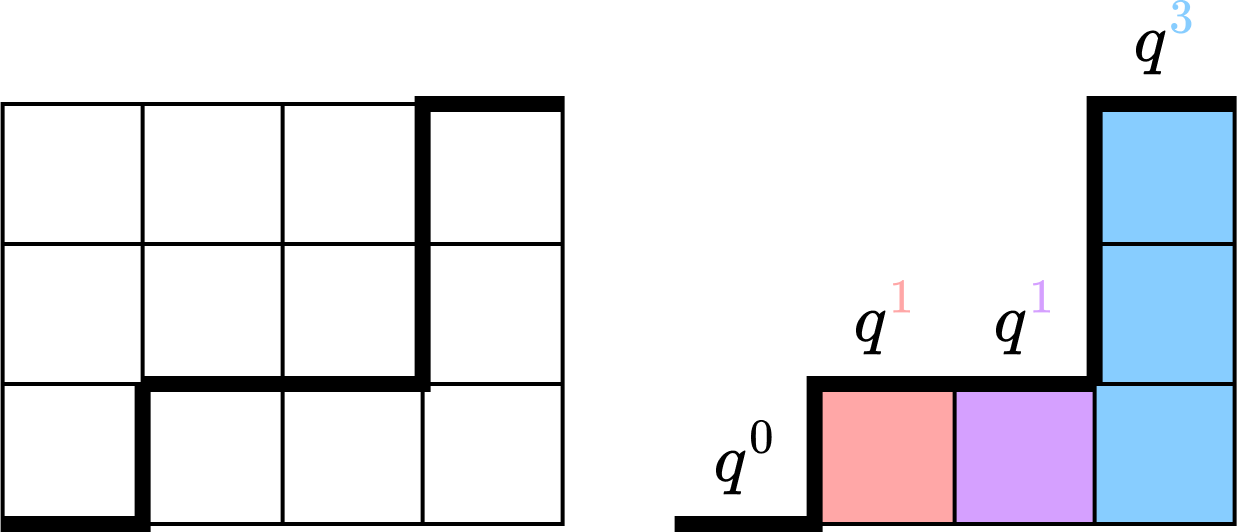
\includegraphics[width=0.65\linewidth]{Images/Figure27.png}
    \caption{A lattice path with weight $q^0q^1q^1q^3=q^5$.}
    \label{f:F2L}
\end{figure}
We want to give a $q$-analogue of the double counting argument we used in \cref{q:1.8} to come up with a useful recurrence. 
\begin{figure}[H]
    \centering
    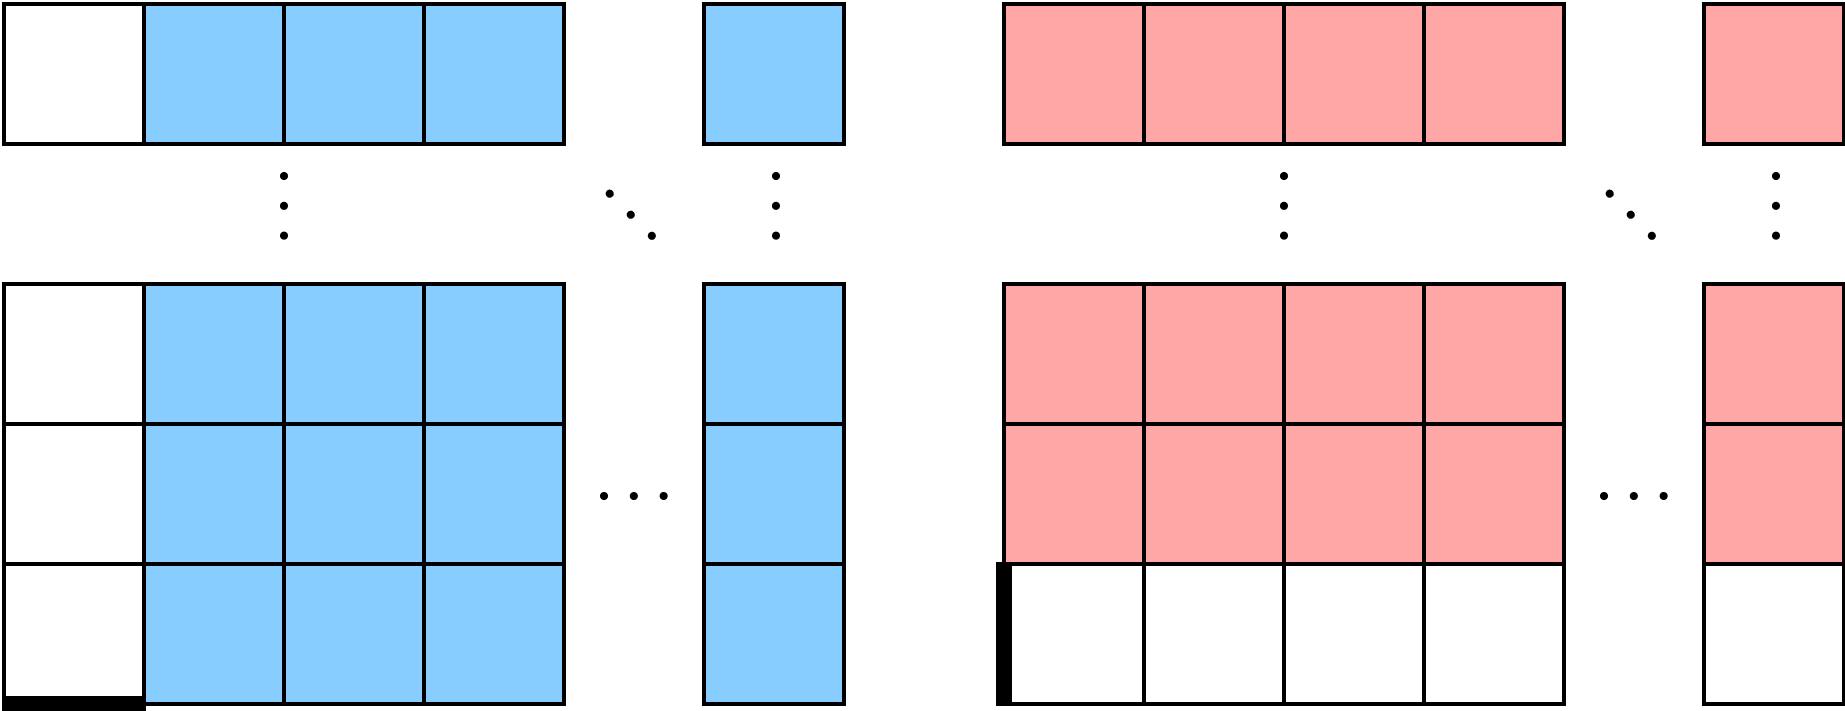
\includegraphics[width=0.65\linewidth]{Images/Figure28.png}
    \caption{}
    \label{fig:Cayley_Rec}
\end{figure}
Refer to \cref{fig:Cayley_Rec} and notice how if a lattice path starts with an $E$-step then we only have to care about the weights due the ``smaller'' path over the remaining blocks (colored blue). On the other hand, if a lattice path starts with an $N$-step then we first row (colored white) always adds a weight of $1$ block and we only have to take care of the ``smaller'' lattice path over the remaining blocks (colored red). Putting \cref{c:q_Pascal} and our observation together allows us to deduce the following result due to George Polya.
\begin{theorem}
Let $A_{n,k}(r)$ denote the number of $n$-step lattice paths from $(0,0)$ to $(k,n-k)$ which span $r$ unit blocks under them. Then 
\[
\binom{n}{k}_q = \sum_{r=0}^{k(n-k)}A_{n,k}(r)q^r
\]
\end{theorem}
It is not difficult to see that every lattice path corresponds to a Ferrer's diagram and hence a partition. For instance, the lattice path in \cref{f:F2L} corresponds to the partition $3+1+1$ of $5$. To this end, consider the following theorem due to Cayley.
\begin{theorem}
Let $p_{i,j}\left( n \right)$ denote the number of partitions of $n$ into atmost $i$ parts each of which is atmost $j$. Then \[
	\sum_{n=0}^{ij}p_{i,j}\left( n \right) q^n = \binom{i+j}{i}_q 
\]     
\end{theorem}
\begin{proof}
Let $c_{i,j}\left( n \right)$ denote the number of sequences with $i$-many $0$s and $j$-many $1$s having exactly $n$-many inversions. We know that
\begin{align*}
	\binom{i+j}{i}_q = \sum_{n=0}^{ij}c_{i,j}\left( n \right)q^n.
\end{align*}
Also, if $A_{i,j}\left( n \right)$ denotes the number of lattice paths from $\left( 0,0 \right)$ to $\left( i,j \right)$ we also know that
\begin{align*}
	\binom{i+j}{i}_{q} = \sum_{n=0}^{ij}A_{i,j}\left( n \right)q^n.
\end{align*}
Hence, to prove our claim it suffices to construct a bijection between $p_{i,j}\left( n \right)$ and $A_{i,j}\left( n \right)$ and/or $c_{i,j}\left( n \right)$. To this end, consider the following partition \[
	n = \pi_{1}+\pi_{2}+\cdots+\pi_{i}
\]
where $\pi_{k}\leq j$ for all possible choices of $k$. For every such partition, it is possible to construct a sequence of $j$-many $0$s and $i$-many $1$s, say $\sigma$, which has exactly $\pi_{1}$-many $0$s followed by the first occurrence of $1$ in $\sigma$, $\pi_{2}$-many $0$s followed by the second occurrence of $1$ in $\sigma$, and so on, all the way up to $\pi_{i}$-many $0$s followed by the last occurrence of $1$ in $\sigma$. This gives a bijection between $p_{i,j}\left( n \right)$ and $c_{j,i}\left( n \right)$. Next, we give a bijection between $p_{i,j}\left( n \right)$ and $A_{i,j}\left( n \right)$. Let $\sigma \in S\left(j,i\right)$ be the sequence of $j$-many $0$s and  $i$-many $1$s corresponding to the partition of $n$ considered above. Now, setting the occurrence of a $1$ in $\sigma$, and the occurrence of a $0$ in $\sigma$ to an $N$ move, and an $E$ move respectively in the Ferrers diagram of $\pi_{1}+\cdots+\pi_{i}$ gives a path from $\left( 0,0 \right)$ to $\left( i,j \right)$ which spans exactly $n$ blocks under it.
\end{proof}
We conclude this section by introducing two different $q$-analogues of Catalan numbers. Before doing so we introduce a new statistic on permutations. 
\begin{definition}
Let $\sigma$ be a permutation on $[n]$. An integer $1\leq i\leq n-1$ is called a descent of $\sigma$ if $\sigma(i)>\sigma(i+1)$. 
\end{definition}
The set of all descents of a permutation is called it's descent set. For instance the descent set of $(613524)$ is $\{1,4\}$. Finally, the major index of a permutation is the sum of all the elements in the descent set. These definitions might seem unmotivated. However, consider the following result which we state without a proof (one proof is outlined as an exercise in Assignment 3). 
\begin{theorem}
Let $S_n$ denote the set of all permutations on $[n]$. Let $\text{maj}(\sigma)$ denote the major index of a permutation $\sigma$ in $S_n$. Then
\[
    \sum_{\sigma\in S_n} q^{\text{maj}(\sigma)} = n!_q.
\]
\end{theorem}
With this background at hand, we are ready to introduce a $q$-analogue of Catalan numbers first given by MacMahon.
\begin{theorem}
Let $L^+$ denote the set of all lattice paths from $(0,0)$ to $(n,n)$ which never go below the main diagonal. For an arbitrary choice of $\pi\in L^+$, let $\sigma(\pi)$ denote the $2n$-length sequence obtained by replacing each occurrence of an $N$ with $0$ and each occurrence of an $E$ with a $1$. Then 
    \[
    \sum_{\pi\in L^+} q^{\text{maj}(\sigma(\pi))} = \dfrac{1}{[n+1]_q}\binom{2n}{n}_q
    \]
\label{t:qCat1}
\end{theorem}
\begin{proof}
\end{proof}
We present yet another natural $q$-analogue of Catalan numbers, one which satisfies a recurrence relation similar to \cref{t:segner}. Per usual, we start with a definition.
\begin{definition}
    Let $L^+$, $\pi$ and $\sigma(\pi)$ be as defined in the setting of \cref{t:qCat1}. By $\text{area}(\pi)$ we refer to sum of the components of the vector obtained by counting the number of complete unit squares to the right at the occurrence of each $N$ step in $\pi$.
\end{definition}
\begin{figure}[H]
    \centering
    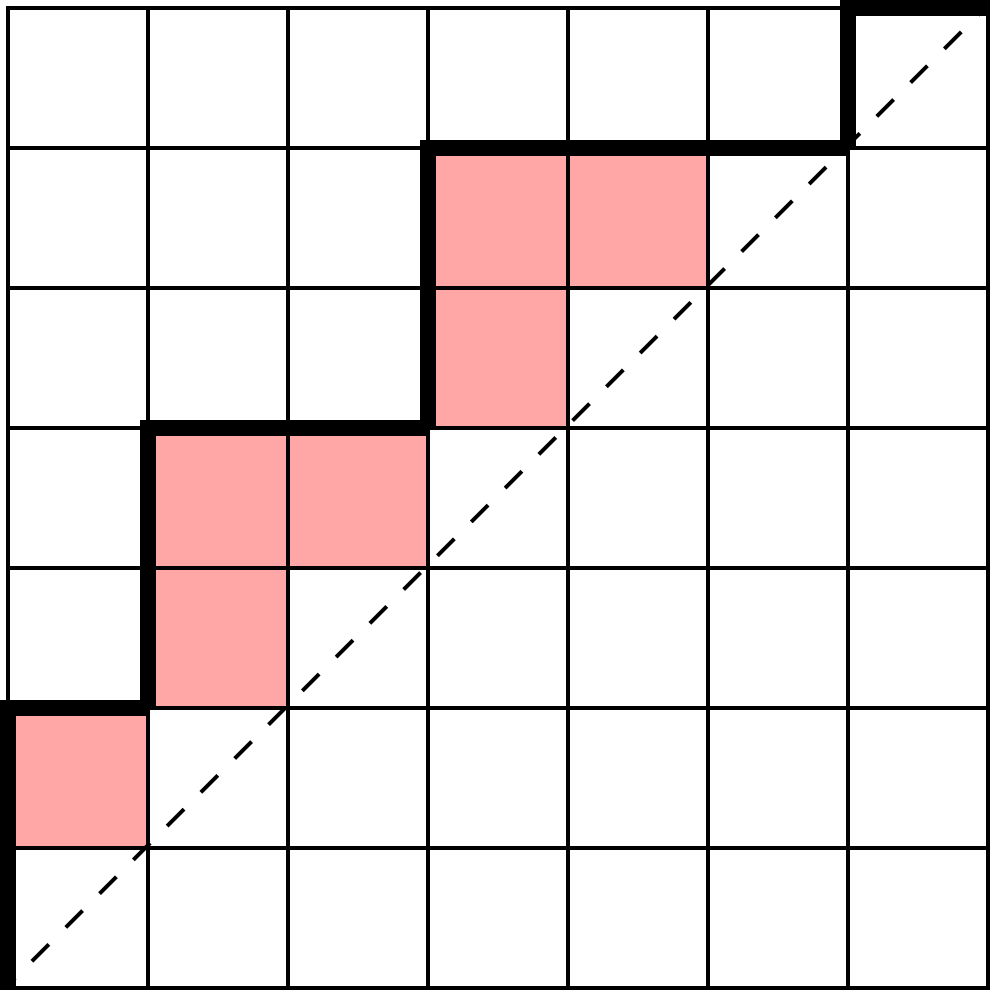
\includegraphics[width=0.5\linewidth]{Images/Figure31.png}
    \caption{An example of a path in $L^+$ with area vector $(1,1,2,1,2)$ and area $1+1+2+1+2=7$.}
    \label{fig:enter-label}
\end{figure}
Now, by a result due to Carlitz and Riordan we have.
\begin{theorem}
    If we set $C_n(q)=\sum_{\pi\in L^+}q^{\text{area}(\pi)}$, then \[
    C_n(q) = \sum_{k=1}^n q^{k-1} C_k(q) C_{n-k}(q).
    \]
\end{theorem}
\begin{proof}
\end{proof}
\endinput
